%%%%%%%%%%%%%%%%%%%%%%%%%%%%%%%%
% Section 5. Application: DAPO with RSP
%%%%%%%%%%%%%%%%%%%%%%%%%%%%%%%%

\section{Application: DAPO Training with RSP}\label{sec:application}

The empirical analysis so far evaluates RSP at inference time only. Section~\ref{sec:multipath} predicts that independent RSP draws should benefit any sampling-based optimization that depends on rollout diversity. We test this prediction by integrating RSP into a GRPO-based RL training pipeline. Implementation details and full per-step results are deferred to Appendix~\ref{app:dapo}.

\paragraph{DAPO.}
DAPO \citep{yu2025dapo} extends GRPO \citep{shao2024deepseekmath} with loss-term modifications that preserve rollout diversity during long chain-of-thought RL training. The diversity is shaped at the loss level by reshaping how rollouts are weighted and clipped. RSP, in contrast, induces diversity at the input level by perturbing the rollout distribution before any loss is computed (Section~\ref{sec:diversity}). We use DAPO as a testbed to ask whether these two diversity sources compose to yield further performance gains. Let $o_i$ be the $i$-th rollout response, $r_{i,t}(\theta) = \pi_\theta(o_{i,t}\mid q, [\mathbf{H}_g,] o_{i,<t}) / \pi_{\theta_{\text{old}}}(o_{i,t}\mid q, [\mathbf{H}_g,] o_{i,<t})$ the importance ratio, $\hat{A}_{i,t}$ the group-relative advantage, and $(\varepsilon_{\text{low}}, \varepsilon_{\text{high}})$ the asymmetric clip range. The bracketed $\mathbf{H}_g$ is the RSP appended to the prompt. The DAPO + RSP objective is
\begin{equation}\label{eq:dapo_rsp}
\mathcal{J}_{\text{DAPO+RSP}}(\theta)
\;=\;
\mathbb{E}\!\left[
\frac{1}{\sum_i |o_i|}
\sum_{i,t}
\min\!\Big(r_{i,t}\hat{A}_{i,t},\,
\text{clip}\big(r_{i,t},\,1{-}\varepsilon_{\text{low}},\,1{+}\varepsilon_{\text{high}}\big)\hat{A}_{i,t}\Big)
\right].
\end{equation}

\paragraph{Setup.}
We train Qwen2.5-Math-7B on a MATH Level-3--5 subset (\textasciitilde 8.5K prompts) using the SimpleRL-Zoo \citep{zeng2025simplerl} training pipeline with the objective of Eq.~\eqref{eq:dapo_rsp}. Each step samples $G=8$ rollouts per prompt over a batch of $1{,}024$ prompts under $\tau{=}1.0$, for $100$ training steps (approximately $12$ epochs). We compare \emph{DAPO} against \emph{DAPO + RSP}, where RSP suffix injection ($L=20$ tokens) is applied during rollouts only; evaluation is performed without RSP. We evaluate on seven mathematical-reasoning benchmarks (MATH-500 \citep{lightman2024lets}, AIME 2024, AMC 2023, GSM8K \citep{cobbe2021training}, GaoKao 2023-EN, OlympiadBench \citep{he2024olympiad}, Minerva Math \citep{lewkowycz2022minerva}). The small competition sets (AIME 2024, AMC 2023) are scored by Avg@32 at $\tau{=}1.0$ to reduce variance, while the larger benchmarks use greedy single-sample evaluation. We report the unweighted seven-benchmark average.

\paragraph{Results.}
Figure~\ref{fig:dapo_curve} shows the seven-benchmark average accuracy across training steps, and Table~\ref{tab:dapo_peak} reports per-benchmark accuracy at each method's peak step.

\begin{table}[!ht]
\centering
\caption{Per-benchmark accuracy (\%) at each method's peak step on Qwen2.5-Math-7B. \textbf{Bold} denotes the better of the two RL methods on each benchmark. Avg is the unweighted seven-benchmark mean.}
\label{tab:dapo_peak}
\footnotesize
\setlength{\tabcolsep}{4pt}
\renewcommand{\arraystretch}{0.9}
\begin{tabular}{l ccccccc c}
\toprule
\textbf{Method} & \textbf{MATH-500} & \textbf{AIME 24} & \textbf{AMC 23} & \textbf{GSM8K} & \textbf{GaoKao 23-EN} & \textbf{Olymp.} & \textbf{Minerva} & \textbf{Avg} \\
\midrule
Base                & 52.6 & 8.6  & 23.9 & 57.2 & 38.7 & 16.3 & 13.6 & 30.13 \\
DAPO                & 78.2 & 22.6 & \textbf{62.2} & 86.3 & \textbf{62.6} & \textbf{38.5} & 37.5 & 55.41 \\
\rowcolor{blue!10}
DAPO~+~RSP          & \textbf{78.6} & \textbf{23.6} & \textbf{62.2} & \textbf{87.7} & \textbf{62.6} & \textbf{38.5} & \textbf{39.7} & \textbf{56.13} \\
\bottomrule
\end{tabular}
\end{table}

\paragraph{Interpretation.}
\begin{wrapfigure}{r}{0.42\textwidth}
  \vspace{-1.0em}
  \centering
  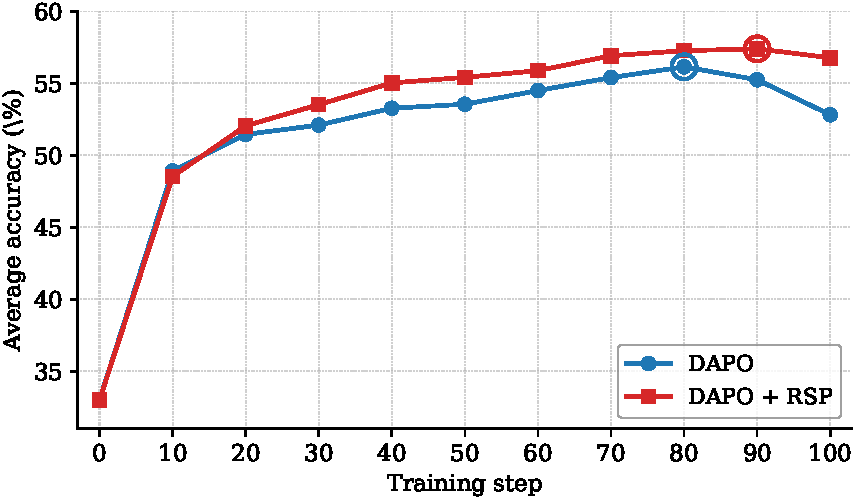
\includegraphics[width=0.40\textwidth]{img/dapo/dapo_avg_curve.pdf}
  \caption{Seven-benchmark average accuracy on Qwen2.5-Math-7B. DAPO~+~RSP reaches a higher peak (step~90) and stays stable through step~100, while DAPO declines after step~80.}
  \label{fig:dapo_curve}
\end{wrapfigure}
Two patterns emerge. First, DAPO alone peaks at step~80 (55.41\%) and then declines, reaching 52.56\% by step~100; DAPO~+~RSP keeps climbing to a 56.13\% peak at step~90 and stays at 55.81\% by step~100. This is consistent with input-space resampling acting as a \emph{complementary} source of diversity to DAPO's loss-level entropy management: RSP injects independent perturbations across rollouts and does not depend on the policy's own entropy. Second, the peak itself improves modestly (+0.72\,pp average), so RSP both \emph{delays collapse} and \emph{raises the attainable performance}. Both patterns are facets of the same mechanism: RSP's early-stage branch opening (Section~\ref{sec:multipath}), the classical exploration--exploitation pattern in RL \citep{sutton2018reinforcement}, slows reward growth at first (the two curves cross around step~20) but compounds into both delayed collapse and a higher peak. We treat this as preliminary evidence that input-space and loss-level diversity mechanisms compose; limitations and broader robustness checks are discussed in Appendix~\ref{app:dapo_limitations}.
